%%%%%%%%%%%%%%%%%%%%%%%%%%%%%%%%%%%%%%%%%%%%%%%%%%%%%%%%%%%%%%%%%
% Contents : The planned transactions chapter
% $Id : grisbi-manuel-planned.tex, v 0.4 2002/10/27 Daniel Cartron
% $Id : grisbi-manuel-planned.tex, v 0.5.0 2004/06/01 Loic Breilloux
% $Id : grisbi-manuel-planned.tex, v 0.6.0 2011/11/17 Jean-Luc Duflot
% $Id : grisbi-manuel-planned.tex, v 0.8.9 2012/04/27 Jean-Luc Duflot
% $Id : grisbi-manuel-planned.tex, v 1.0 2014/02/12 Jean-Luc Duflot
%%%%%%%%%%%%%%%%%%%%%%%%%%%%%%%%%%%%%%%%%%%%%%%%%%%%%%%%%%%%%%%%%

\chapter{Échéancier\label{plannedtransactions}}

L'échéancier permet de planifier des opérations qui reviennent régulièrement avec des dates ou des intervalles de temps déterminés. Une fois qu'une opération est enregistrée dans l'échéancier, Grisbi recopie automatiquement l'opération planifiée dans la liste des opérations dès que sa \indexword{date d'échéance}\index{date !échéance} est atteinte. 

De plus, Grisbi affiche dans la page d'accueil des alertes au déclenchement des échéances de ces opérations (voir la section \vref{home-details-homepage}, \menu{Affichage de la page d'accueil}.

% espace pour changement de thème
\vspacepdf{5mm}
Pour planifier des opérations, cliquez sur \menu{Échéancier} dans le panneau de navigation, ou sélectionnez \menu{Opérations Planifiées} avec la barre d'information (voir le chapitre \vref{home}, \menu{Accueil}).

Un calendrier s'affiche en bas du panneau de navigation, et le pavé des détails possède alors trois éléments :
\begin{itemize}
	 \item la barre d'outils ;
	 \item la liste des opérations planifiées ;
	 \item le formulaire de saisie des opérations planifiées.
\end{itemize}

% espace pour changement de thème
\vspacepdf{5mm}
Vous pouvez configurer les paramètres des alertes de l'échéancier dans le menu \menu{Édition - Préférences} (voir la section \vref{setup-general-planned}, \menu{Échéancier}).


\section{Barre d'outils\label{plannedtransactions-functions}}


La barre d'outils des opérations planifiées présente les fonctions suivantes : 

\begin{itemize}
	 \item \menu{Nouvelle Échéance} : ouvre le formulaire de saisie vierge ;
	 \item \menu{Supprimer} : supprime l'opération planifiée sélectionnée ;
	 \item \menu{Éditer} : ouvre le formulaire de saisie pour l'opération sélectionnée et permet de la modifier ;
	 \item \menu{Remarques} ou \menu{Périodicité/Mode} : affiche la colonne \menu{Remarques} à la place des colonnes \menu{Périodicité} et \menu{Mode}, ou inversement ; 
	 \item \menu{Exécuter} : exécute l'opération planifiée sélectionnée, c'est-à-dire la recopie dans la liste des opérations du compte concerné ;
	 \item \menu{Affichage} : une liste déroulante permet de choisir l'affichage des opérations planifiées : toutes, selon diverses périodicités, ou selon un réglage personnalisé.
\end{itemize}

% espace pour changement de thème
\vspacepdf{5mm}
La barre d'outils peut être déplacée dans l'écran en cliquant sur sa poignée (petit rectangle vertical à gauche de la barre) et en la déplaçant. Pour la réattacher à son emplacement d'origine dans le pavé des détails, la remettre en haut de la fenêtre, le haut de la poignée sur le petit trait qui visualise sa place d'origine.

% saut de page pour titre solidaire
\ifIllustration
\newpage
\fi


\section{Liste des opérations planifiées\label{plannedtransactions-list}}


\subsection{Description\label{plannedtransactions-list-description}}

La liste des opérations planifiées s'affiche dans le panneau des
\ifIllustration détails\refimage{planned-transactions-list-img}.
\else détails.
\fi

% image centrée
\ifIllustration
\begin{figure}[htbp]
\begin{center}
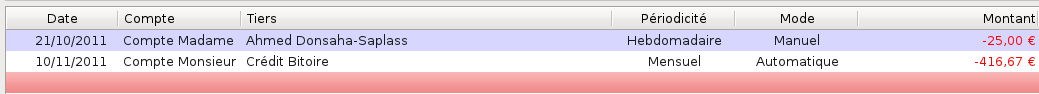
\includegraphics[scale=0.5]{image/screenshot/planned_transactions_list}
\end{center}
\caption{Liste des opérations planifiées}
\label{planned-transactions-list-img}
\end{figure}
% image centrée
\fi

Elle affiche en haut la barre des libellés des colonnes. Vous pouvez \indexword{élargir ou rétrécir une colonne}\index{colonne !largeur} en cliquant sur le séparateur entre deux colonnes et en le déplaçant. Pour rétablir la \indexword{largeur des colonnes}\index{colonne !largeur} à leur valeur par défaut, sélectionnez le menu \menu{Affichage - Réinitialiser la largeur des colonnes}.

Vous pouvez déplacer la liste des opérations planifiées vers le haut ou vers le bas avec la molette de la souris, ou bien avec la souris et l'ascenseur vertical. Le déplacement éventuel vers la gauche ou la droite se fait avec la souris et l'ascenseur horizontal.

% espace pour changement de thème
\vspacepdf{5mm}
Chaque opération est affichée sur une seule ligne et au maximum six colonnes, ce qui fait au maximum six champs d'information pour chaque opération planifiée. Les champs d'affichage, ainsi que les \indexword{libellés des colonnes}\index{colonne !libellé}, sont les suivants :
\begin{itemize}
	 \item \menu{Date} : la date de l'opération ;
	 \item \menu{Compte} : le compte concerné ;
	 \item \menu{Tiers} ;
	 \item \menu{Périodicité} : la périodicité de l'opération ;
	 \item \menu{Mode} : le mode d'exécution, automatique ou manuel ; 
	 \item \menu{Montant} : le montant de l'opération ; un \indexword{montant négatif}\index{montant !négatif} est affiché en rouge{\couleur}.
% saut de ligne pour indentation correcte de la note dans la liste

\textbf{Note} : si l'affichage du champ \menu{Remarques} a été demandé, il s'affiche à la place des champs \menu{Périodicité} et \menu{Mode}, ce qui ne fait plus que cinq colonnes et cinq champs affichés.	 
\end{itemize}

% espace pour changement de thème
\vspacepdf{5mm}
Une ligne supplémentaire vide s'affiche juste en-dessous de la dernière ligne d'opération, et sert à créer une nouvelle opération planifiée (voir la section \vref{plannedtransactions-new}, \menu{Nouvelle opération planifiée}).

% espace pour changement de thème
\vspacepdf{5mm}
Pour des raisons de lisibilité de l'affichage, Grisbi présente une alternance de couleurs de fond violet et blanc{\couleurs} à chaque ligne.

% espace pour changement de thème
\vspacepdf{5mm}
En cliquant sur l'outil  \menu{Affichage} dans la barre d'outils, une liste déroulante vous permet de choisir plusieurs modes d'affichage des prochaines occurrences :
% espace avant image 5mm
\vspacepdf{3mm}

\begin{itemize}
	\ifIllustration
	% image entourée par une liste (picins)
	% pas de référence à l'illustration car erreur de numéro de figure avec picins.
	% supprimé car en html les figures entourées ne sont pas numérotées, et la numérotation des figures centrées décalée par rapport au pdf
	%\piccaption{Choix des modes d'affichage}
	\label{planned-transactions-display-img}
	\parpic[r]{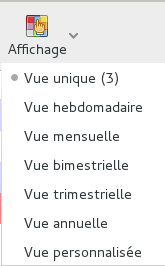
\includegraphics[scale=0.50]{image/screenshot/planned_transactions_display}}
	% image entourée par une liste (picins)
	\fi
	 \item \menu{Vue unique} : la prochaine occurrence de chaque opération ; 
	 \item \menu{Vue hebdomadaire} ; à échéance de 7 jours ;
	 \item \menu{Vue mensuelle} : à échéance de 30 jours ;
	 \item \menu{Vue bimestrielle} : à échéance de 60 jours  ;
	 \item \menu{Vue trimestrielle} : à échéance de 90 jours  ;
	 \item \menu{Vue annuelle} : à échéance d'un an ;
	 \item \menu{Vue personnalisée} : à échéance d'un nombre quelconque de jours, semaines, mois ou années.
% espace pour Note ou Attention à la ligne dans une liste

	 % espace pour changement de thème
	 \vspacepdf{3mm}   
	 L'affichage courant y est indiqué par une coche, ainsi que le nombre d'opérations dans cette vue.
\end{itemize}

\ifIllustration
% espace après image entourée
\vspacepdf{13mm}
\vspacehevea{7mm}
\else
\vspacepdf{5mm}
\fi

Si vous choisissez l'affichage personnalisé, une nouvelle fenêtre affiche deux listes déroulantes pour choisir le nombre et la période \ifIllustration désirés\refimage{planned-transactions-display-custom-img}.

% image centrée 
\begin{figure}[htbp]
\begin{center}
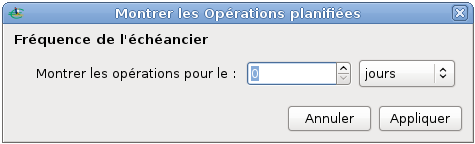
\includegraphics[scale=0.5]{image/screenshot/planned_transactions_display_custom}
\end{center}
\caption{Choix de l'affichage de la période personnalisée}
\label{planned-transactions-display-custom-img}
\end{figure}
% image centrée 
\else désirés.
\fi

\ifIllustration
\else
% saut de page pour titre solidaire
\newpage
\fi


\subsection{Tris\label{plannedtransactions-list-sorts}}

Pour changer l'ordre d'affichage des opérations planifiées, vous pouvez faire un \indexword{tri sur les opérations}\index{tri !opérations} sur un des champs d'information ; procédez comme suit :

\begin{enumerate}
	  \item cliquez sur le libellé de la colonne qui contient le champ d'information choisi comme critère de \gls{tri} ; les seuls critères de tri possibles sont la \menu{Date}, le \menu{Compte} et le \menu{Tiers}.
	  \item toutes les opérations s'affichent, triées selon le critère choisi ;
	  \item un petit triangle noir apparaît à droite du libellé de la colonne ; il pointe vers le bas si le tri est ascendant, vers le haut si le tri est descendant ;

\textbf{Note} : ces triangles peuvent être remplacés, en fonction du thème de l'environnement de bureau ou du gestionnaire de fenêtres que vous utilisez, par d'autres caractères tels que +, -, >, <, etc.
	  \item cliquez sur ce triangle pour changer l'ordre du tri.
\end{enumerate}


\section{Formulaire de saisie des opérations planifiées\label{plannedtransactions-form}}


Le formulaire de saisie des opérations planifiées s'affiche en-dessous de la liste des opérations planifiées. Il est similaire au formulaire de saisie des opérations ordinaires, mais il comprend, dans sa partie supérieure, une ligne supplémentaire de trois à six champs pour \ifIllustration indiquer\refimage{planned-transactions-form-img} :
\else indiquer :
\fi

\ifIllustration
% image centrée
\begin{figure}[htbp]
\begin{center}
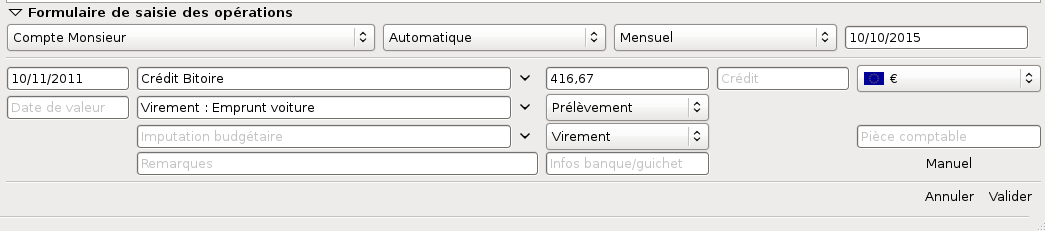
\includegraphics[scale=0.5]{image/screenshot/planned_transactions_form}
\end{center}
\caption{Formulaire de saisie des opérations planifiées}
\label{planned-transactions-form-img}
\end{figure}
% image centrée
\fi

\begin{itemize}
	\item le compte affecté ; dans le cas d'un virement entre deux comptes, vous pouvez sélectionner l'un ou l'autre des deux comptes (origine ou destination) ; le type de l'opération (débit ou crédit) doit être renseigné dans le champ adéquat, et la contre-opération sera automatiquement créée dans l'autre compte au moment de l'exécution de l'opération planifiée ;
	
	\item le mode d'exécution :
	
		\begin{itemize}
			\item \menu{Manuel} : vous devrez exécuter manuellement la saisie dans le formulaire en sélectionnant la fonction \menu{Exécuter} dans la barre de fonctions ou dans le menu contextuel (voir la section \vref{plannedtransactions-execution}, \menu{Exécution d'une opération planifiée},
			\item \menu{Automatique} : l'opération sera automatiquement saisie dans la liste des opérations à la date programmée ;
		\end{itemize}
	
	\item la \menu{Périodicité} :
		\begin{itemize}
			\item \menu{Une fois},
			\item \menu{Hebdomadaire},
			\item \menu{Mensuelle},
			\item \menu{Bimestrielle},
			\item \menu{Trimestrielle},
			\item \menu{Annuelle},
			\item \menu{Personnalisée} ; dans ce cas, vous devrez préciser plus finement le nombre de périodes entre chaque saisie ou demande de validation de l'opération, ainsi que la période voulue (jours, semaines, \ifIllustration mois, années)\refimage{planned-transactions-frequency_custom-img} ;
	\else mois, années) ;
	\fi
	
	\ifIllustration
	% image centrée
	\begin{figure}[htbp]
	\begin{center}
	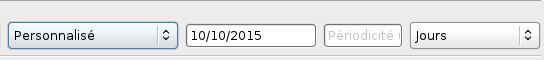
\includegraphics[scale=0.5]{image/screenshot/planned_transactions_frequency_custom}
	\end{center}
	\caption{Saisie d'une périodicité personnalisée}
	\label{planned-transactions-frequency_custom-img}
	\end{figure}
	% image centrée
	\fi
	\end{itemize}
\item la \menu{Date limite} des échéances ; le choix par défaut est \menu{Aucune} ; un double-clic ou la combinaison de touches \key{Ctrl}\key{Entrée} dans ce champ ouvre un calendrier (voir la section \vref{plannedtransactions-calendar}, \menu{Calendrier et prévisions}) ; vous pouvez aussi saisir manuellement la date en utilisant les multiples combinaisons de touches telles que décrites dans la section \vref{transactions-new-dates}, \menu{Saisie de date au clavier}.
\end{itemize}

% espace pour changement de thème
\vspacepdf{5mm}
La partie inférieure du formulaire est strictement identique au formulaire de saisie des opérations ordinaires, et est géré de la même manière \ifIllustration \refimage{planned-transactions-form-img},
\else manière,
\fi
 voir la section \vref{transactions-form}, \menu {Formulaire de saisie}.

% espace pour changement de thème
\vspacepdf{5mm}
Une fois le formulaire affiché, un menu contextuel accessible par un clic-droit dans un champ de saisie permet d'effectuer les actions suivantes :

\begin{itemize}
	 \item \menu{Couper} (la sélection) ;
	 \item \menu{Copier} (la sélection) ;
	 \item\menu{Coller} (la sélection) ;
	 \item \menu{Supprimer} (la sélection) ;
	 \item \menu{Tout sélectionner} (dans le champ de saisie) ;
	 \item \menu{Méthodes de saisie} ;
	 \item \menu{Insérer un caractère de contrôle Unicode}.
\end{itemize}

Le choix \menu{\gls{methodes de saisie}} permet de changer les caractères accentués.

Le choix \menu{Insérer un \gls{caractere de controle Unicode}} permet d'insérer un code Unichar qui modifie la présentation ; par exemple RLO (forçage droite-à-gauche) renverse l'ordre des lettres et la position du texte.

% espace pour changement de thème
\vspacepdf{5mm}
De plus, un autre menu contextuel accessible par un clic-droit dans le formulaire de saisie, dans une zone grise en dehors des champs de saisie, permet d'accéder à la configuration du formulaire, en sélectionnant  \menu{Configurer le formulaire} (voir la section \vref{setup-form}, \menu{Formulaire des opérations}).

% espace pour changement de thème
\vspacepdf{5mm}
Notez que le choix des types d'opérations est nécessairement lié au type du compte sélectionné (voir la section \vref{accounts-type}, \menu{Types de compte de Grisbi}).


\section{Calendrier et prévisions\label{plannedtransactions-calendar}}


Un calendrier s'affiche à la place du bas du panneau de navigation. Il indique en caractères gras les dates auxquelles des opérations planifiées de tous les comptes arrivent à échéance, et sur fond bleu{\couleur} la date du jour.

Cliquez sur le calendrier pour le sélectionner. Vous pouvez le parcourir avec la souris ou le clavier :
% espace avant image 5mm
\vspacepdf{3mm}

\begin{itemize}
	% image entourée par une liste ( picins)
	% pas de référence à l'illustration car erreur de numéro de figure avec picins.
	\ifIllustration
	% supprimé car en html les figures entourées ne sont pas numérotées, et la numérotation des figures centrées décalée par rapport au pdf
	%\piccaption{Calendrier des opérations planifiées}
	\label{planned-transactions-calendar-img}
	\parpic[r]{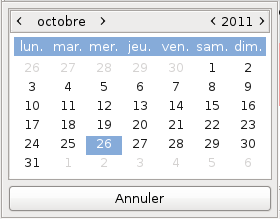
\includegraphics[scale=0.5]{image/screenshot/planned_transactions_calendar}}
	% image entourée par une liste ( picins)
	\fi
	
	\item les touches \key{Flèche Gauche} ou \key{Flèche Droite}, permettent de passer au jour précédent ou suivant ;
	\item les touches \key{Flèche Haut} ou \key{Flèche Bas} permettent de passer à la semaine précédente ou suivante ;
	\item la combinaison de touches \key{Ctrl}\key{Flèche Gauche} ou \newline \key{Ctrl}\key{Flèche Droite} permet de passer au mois précédent ou suivant ;
	\item la combinaison de touches \key{Ctrl}\key{Flèche Haut} ou \newline \key{Ctrl}\key{Flèche Bas} permet de passer à l'année précédente ou suivante.
\end{itemize}

\ifIllustration
% espace après image entourée
\vspacepdf{5mm}
\vspacehevea{10mm}
\fi


\section{Sélection d'une opération planifiée\label{plannedtransactions-selection}}


Pour sélectionner une opération planifiée, vous avez deux moyens :

\begin{itemize}
	 \item cliquer sur sa ligne ;
	 \item déplacer la sélection avec les touches du clavier \key{Flèche Haut} et \key{Flèche Bas}.
\end{itemize}

L'opération apparaît alors sur fond bleu{\couleur} et ses détails s'affichent dans le formulaire.

% espace pour changement de thème
\vspacepdf{5mm}
Un menu contextuel est disponible sur la liste des opérations planifiées. Un clic-droit sur la ligne d'une opération permet les fonctions suivantes, selon le contexte :
% espace avant image 5mm
\vspacepdf{3mm}

\begin{itemize}
	% image entourée par une liste (picins)
	% pas de référence à l'illustration car erreur de numéro de figure avec picins.
	\ifIllustration
	% supprimé car en html les figures entourées ne sont pas numérotées, et la numérotation des figures centrées décalée par rapport au pdf
	%\piccaption{Menu contextuel de la liste des opérations planifiées}
	\label{planned-transactions-context-img}
	\parpic[r]{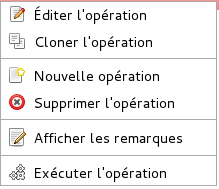
\includegraphics[scale=0.5]{image/screenshot/planned_transactions_context}}
	% image entourée par une liste (picins)
	\fi
	 \item \menu{Éditer l'opération} ;
	 \item \menu{Cloner l'opération} ;
	 \item \menu{Nouvelle opération} ;
	 \item \menu{Supprimer l'opération} ;
	 \item \menu{Afficher les remarques} ;
	 \item \menu{Afficher Périodicité/Mode} ;	 
	 \item \menu{Exécuter l'opération}.
\end{itemize}

\ifIllustration
% espace après image entourée
\vspacepdf{11mm}
\fi


\section{Nouvelle opération planifiée\label{plannedtransactions-new}}


La saisie d'une opération planifiée se fait d'une manière similaire à la saisie d'une opération ordinaire.

Vous pouvez ouvrir le formulaire de saisie avec l'une de ces méthodes :

\begin{itemize}
	 \item sélectionnez la ligne vide en bas de la liste des opérations et appuyez sur la touche \key{Entrée} ;
	 \item double-cliquez sur la ligne vide ;
	 \item dans la barre d'outils, cliquez-gauche sur l'outil \menu{Nouvelle échéance} ;
	 \item dans le menu contextuel, sélectionnez le choix \menu{Nouvelle opération} ;
	 \item cliquez-gauche sur le petit triangle d'affichage/masquage à gauche du libellé \menu{Formulaire de saisie des opérations}, tout en bas du pavé des détails. 
\end{itemize}

\textbf{Note} : ce triangle peut être remplacé, en fonction du thème de l'environnement de bureau ou du gestionnaire de fenêtres que vous utilisez, par d'autres caractères tels que +, -, >, <, etc.

% espace pour changement de thème
\vspacepdf{5mm}
Renseignez les champs avec les paramètres de votre opération planifiée. Pour plus de détails sur la saisie de ces paramètres dans le formulaire, voir les sections \vref{plannedtransactions-form}, \menu{Formulaire de saisie des opérations planifiées} et \vref{plannedtransactions-calendar}, \menu{Calendrier et prévisions}. 


\section{Ventilation d'une opération planifiée\label{plannedtransactions-breakdown}}


La ventilation d'une opération planifiée se fait d'une manière similaire à la ventilation d'une opération ordinaire. Une fois que vous avez renseigné les champs  de la première ligne du formulaire (voir la section \vref{plannedtransactions-form}, \menu{Formulaire de saisie des opérations planifiées}), saisissez les autres paramètres de l'opération dans la partie inférieure de ce formulaire (voir la section \vref{transactions-form}, \menu{Formulaire de saisie}), et procédez à la saisie de l'opération planifiée ventilée, comme décrit précisément dans la section \vref{transactions-breakdown}, \menu{Ventilation d'une opération}.


\section{Modification d'une opération planifiée\label{plannedtransactions-modify}}


Pour modifier une opération planifiée, procédez comme suit :

\begin{enumerate}
	 \item sélectionnez-la dans la liste ;
	 \item cliquez sur l'outil \menu{Éditer} dans la barre d'outils, ou cliquez-droit sur la ligne de l'opération et sélectionnez \menu{Éditer l'opération} dans le menu contextuel ;
	 \item le formulaire de saisie s'ouvre sur le champ  \menu{Date} : vous pouvez alors modifier toutes les données de l'opération ;
	 \item validez par le bouton \menu{Valider}.
\end{enumerate}


\section{Clonage d'une opération planifiée\label{plannedtransactions-duplicate}}


Pour cloner une opération planifiée, sélectionnez-la pour qu'elle s'affiche dans le formulaire de saisie, puis utilisez l'une de ces deux méthodes :

\begin{itemize}
	 \item dans la barre de menus, sélectionnez \menu{Édition - Cloner l'opération} ;
	 \item dans le menu contextuel, sélectionnez \menu{Cloner l'opération}.
\end{itemize}

% espace pour changement de thème
\vspacepdf{5mm}
L'opération sélectionnée précédemment apparaît toujours sur fond  rouge{\couleur}, et l'opération clonée s'affiche dans une nouvelle ligne en-dessous.

Vous pouvez alors éditer cette nouvelle opération, par exemple en modifiant la date.


\section{Remarques des opérations planifiées\label{plannedtransactions-comments}}


Vous pouvez afficher ou cacher les remarques de deux manières :

\begin{itemize}
	 \item cliquez sur l'outil \menu{Remarques} dans la barre d'outils ;
	 \item cliquez-droit sur la ligne de l'opération et sélectionnez \menu{Afficher/Masquer les remarques} dans le menu contextuel.
\end{itemize}

Les remarques de toutes les opérations s'affichent alors à la place des colonnes \menu{Périodicité} et \menu{Mode} dans la liste des opérations planifiées. Recommencer la même séquence réaffiche les colonnes \menu{Périodicité} et \menu{Mode} à la place de la \ifIllustration colonne \menu{Remarques}\refimage{planned-transactions-list-comments-img}.

% image centrée
\begin{figure}[htbp]
\begin{center}
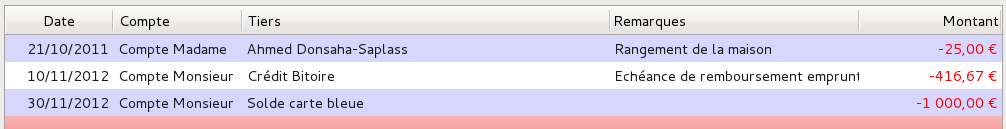
\includegraphics[scale=0.5]{image/screenshot/planned_transactions_list_comments}
\end{center}
\caption{Affichage des remarques des opérations planifiées}
\label{planned-transactions-list-comments-img}
\end{figure}
% image centrée
\else colonne \menu{Remarques}.
\fi

\ifIllustration
% espace après légende 10mm
\vspacepdf{-6mm}
\fi


\section{Exécution d'une opération planifiée\label{plannedtransactions-execution}}


La fonction \menu{Exécuter une opération planifiée} sert uniquement à faire la recopie, dans le formulaire de saisie, de l'occurrence d'une opération sélectionnée dans la liste des opérations planifiées. Pour que cette occurrence soit effectivement transférée dans la liste des opérations du compte concerné, il est nécessaire de valider ensuite le formulaire de saisie, après avoir éventuellement modifié l'opération. 

% espace pour changement de thème
\vspacepdf{5mm}
Pour exécuter une occurrence d'une opération planifiée, procédez comme suit :

\begin{enumerate}
	 \item sélectionnez-la dans la liste ;
	 \item cliquez sur l'outil \menu{Exécuter} dans la barre d'outils, ou cliquez-droit sur la ligne de l'opération et sélectionnez \menu{Exécuter l'opération} dans le menu contextuel ;
	 \item l'occurrence sélectionnée de l'opération s'affiche dans le formulaire de saisie ; vous pouvez alors la modifier selon votre besoin ;
	 \item validez par le bouton \menu{Valider} ; l'occurrence de l'opération est transférée dans la liste des opérations du compte concerné, et la liste des opérations planifiées affiche l'occurrence suivante (si elle existe, car l'opération planifiée peut être unique) de l'opération planifiée. 
\end{enumerate}

% espace avant Attention ou Note  : 5 mm
\vspacepdf{5mm}
\textbf{Note} : après cette validation, la recopie est faite sans autre avertissement.

% espace pour changement de thème
\vspacepdf{5mm}
Vous pouvez aussi vérifier que l'occurrence exécutée de l'opération planifiée se trouve maintenant bien dans  la liste des opérations du compte concerné.


\section{Suppression d'une opération planifiée\label{plannedtransactions-remove}}


Pour supprimer une opération planifiée, procédez comme suit :

\begin{enumerate}
	 \item sélectionnez-la dans la liste ;
	 \item cliquez sur l'outil \menu{Supprimer} dans la barre d'outils, ou cliquez-droit sur la ligne de l'opération et sélectionnez \menu{Supprimer l'opération} dans le menu contextuel ;
	 \item une  boîte de dialogue s'ouvre et vous propose de supprimer, soit toutes les occurrences (toutes les opérations, courante et futures, seront supprimées), soit uniquement l'occurrence courante (seule l'opération \ifIllustration affichée sera supprimée)\refimage{planned-transactions-delete-img} ;
	% image centrée
	\begin{figure}[htbp]
	\begin{center}
	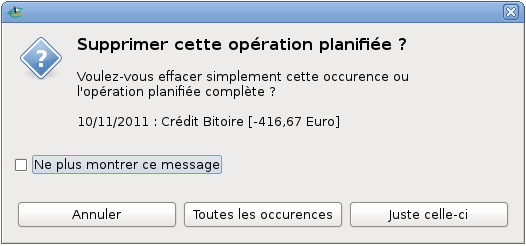
\includegraphics[scale=0.5]{image/screenshot/planned_transactions_delete}
	\end{center}
	\caption{Suppression d'une opération planifiée}
	\label{planned-transactions-delete-img}
	\end{figure}
	% image centrée
	\else affichée sera supprimée) ;
	\fi
	 \item faites votre choix, la suppression est exécutée immédiatement.
\end{enumerate}

 % espace avant Attention ou Note  : 5 mm
\vspacepdf{3mm}
\strong{Attention} : immédiatement après le choix entre \menu{Toutes les occurrences} et \menu{Juste celle-ci}, la suppression est exécutée sans autre avertissement. 

 % espace avant Attention ou Note  : 5 mm
\vspacepdf{4mm}
\strong{Attention} : la suppression d'une opération planifiée est \indexword{irréversible}\index{opération !irréversible} ! 

